\chapter{Tests et Robustesse}

La construction d’un indicateur synthétique repose nécessairement sur un ensemble de choix méthodologiques, notamment en matière d’agrégation et de pondération des variables. Afin d’évaluer la sensibilité des résultats à ces choix, des tests de robustesse ont été menés à l’aide d’une approche par simulation Monte Carlo.

\subsection{Principe général de la simulation Monte Carlo}

Le score de chaque Objectif de Développement Durable (ODD) est initialement calculé comme la moyenne arithmétique des scores de ses indicateurs constitutifs, en supposant une pondération égale. Le score ODD global est ensuite obtenu comme la moyenne arithmétique des scores des différents ODD.

L’analyse de robustesse vise à tester si ces scores restent stables lorsque l’hypothèse de pondération égale est relâchée. Pour ce faire, des pondérations aléatoires sont attribuées aux indicateurs à chaque itération, sous la contrainte que leur somme soit égale à un. À chaque simulation, les scores ODD sont recalculés, puis agrégés afin d’obtenir un score global alternatif. Cette procédure est répétée un grand nombre de fois, ce qui permet d’obtenir une distribution empirique des scores.

\subsection{Robustesse des scores ODD}


Pour chaque ODD, une simulation Monte Carlo a été réalisée en générant 1\,000 combinaisons aléatoires de pondérations appliquées aux indicateurs correspondants. Les distributions obtenues sont présentées sous forme d’histogrammes, accompagnés d’une ligne verticale indiquant le score observé calculé avec pondérations égales.
Il convient de noter que certains Objectifs de Développement Durable, notamment les ODD 13 et 14, reposent sur un nombre très limité d’indicateurs, en l’occurrence un seul indicateur dans le cadre de cette étude. Dans ces conditions, le score de l’ODD correspond directement à la valeur normalisée de l’indicateur considéré, rendant toute analyse de sensibilité fondée sur la variation des pondérations non pertinente. Ces ODD ont ainsi été exclus des tests de robustesse par simulation Monte Carlo au niveau des scores ODD, tout en étant conservés dans le calcul du score ODD global.

Les résultats des simulations montrent que, pour la majorité des ODD, les distributions Monte Carlo sont concentrées autour du score observé, avec des écarts-types généralement modérés. Par exemple, pour l’ODD 1, la moyenne des scores simulés est de 0{,}675, très proche du score initial de 0{,}674, avec un écart-type de 0{,}051 et un intervalle de confiance à 95 \% compris entre 0{,}576 et 0{,}775. De manière similaire, les ODD 2, 3 et 6 présentent des moyennes simulées comprises entre 0{,}648 et 0{,}664, avec des écarts-types inférieurs à 0{,}05, traduisant une faible sensibilité aux variations de pondération des indicateurs.

Certains ODD affichent une robustesse particulièrement élevée. C’est notamment le cas des ODD 11 et 12, dont les écarts-types sont respectivement de 0{,}009 et 0{,}002. Pour ces objectifs, les intervalles de confiance sont très resserrés, indiquant que les scores sont quasi invariants quelle que soit la structure de pondération retenue. À titre illustratif, l’ODD 12 présente un intervalle de confiance à 95 \% compris entre 0{,}964 et 0{,}971, autour d’un score observé de 0{,}967.

À l’inverse, certains ODD se caractérisent par une variabilité plus marquée. Les ODD 7, 16 et 17 présentent des écarts-types supérieurs à 0{,}08, avec des intervalles de confiance relativement larges. Par exemple, l’ODD 17 affiche un intervalle allant de 0{,}472 à 0{,}812, suggérant une sensibilité plus importante du score à la structure de pondération des indicateurs. Cette dispersion plus élevée traduit une hétérogénéité accrue des indicateurs composant ces ODD et appelle à une interprétation plus prudente des scores correspondants.


\begin{figure}[H]
	\centering
	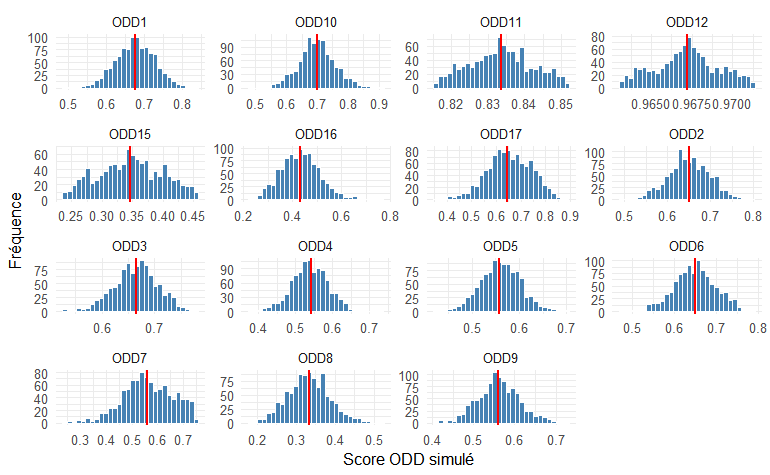
\includegraphics[width=\textwidth]{Pictures/graphs/distribution_MC_ODD.png}
	\caption{Distributions Monte Carlo des scores ODD}
	\label{fig:mc_odd}
\end{figure}

\subsection{Robustesse du score ODD global}

La robustesse du score ODD global a été évaluée en agrégeant, à chaque itération, les scores ODD simulés pour obtenir un score global alternatif. La distribution Monte Carlo du score global est présentée à la Figure \ref{fig:mc_global}.


\begin{figure}[H]
	\centering
	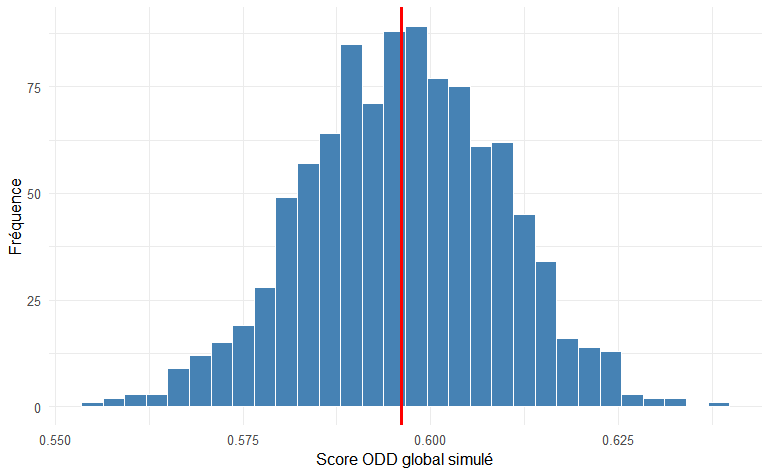
\includegraphics[width=0.85\textwidth]{Pictures/graphs/distribution_MC_global.png}
	\caption{Distribution Monte Carlo du score ODD global}
	\label{fig:mc_global}
\end{figure}

La simulation Monte Carlo appliquée au score ODD global confirme la stabilité de l’indicateur agrégé. La moyenne des scores globaux simulés est de 0{,}5963, pratiquement identique au score global observé de 0{,}5961. L’écart-type associé est faible, de l’ordre de 0{,}013, indiquant une dispersion limitée autour de la valeur centrale.

L’intervalle de confiance empirique à 95 \% du score global s’étend de 0{,}570 à 0{,}621. La position centrale du score observé à l’intérieur de cet intervalle, ainsi que sa proximité avec la moyenne Monte Carlo, suggèrent que le score ODD global est peu sensible aux variations de pondération des indicateurs sous-jacents. Ces résultats confirment que l’agrégation retenue produit un indicateur synthétique stable et représentatif des performances globales.
\subsection{Discussion}

Dans l’ensemble, les résultats des simulations Monte Carlo indiquent que l’indicateur ODD construit présente un niveau de robustesse satisfaisant face aux choix de pondération des indicateurs. Si certains ODD affichent une sensibilité plus marquée, la majorité d’entre eux, ainsi que le score global, demeurent stables lorsque les pondérations varient de manière aléatoire. La faible dispersion observée au niveau du score global suggère en particulier que les incertitudes liées aux pondérations individuelles tendent à se compenser lors de l’agrégation finale. Ces résultats renforcent la solidité méthodologique de l’indicateur et soutiennent son utilisation pour l’analyse comparative et le suivi des performances en matière de développement durable.
